\documentclass[9pt]{article}
\usepackage{array}
\newcolumntype{P}[1]{>{\centering\arraybackslash}p{#1}}
\usepackage{graphicx}
\usepackage[font={small,it}]{caption}
\usepackage{caption}
\usepackage{hyperref}
\usepackage{subfig}
\usepackage[parfill]{parskip}
\usepackage{float}
\usepackage[margin=1in,includefoot]{geometry}
\usepackage{fancyhdr}
\pagestyle{fancy}
\fancyfoot{}

\begin{document}

\begin{titlepage}
\begin{center}
\begin{figure}[t]
\hspace*{0.35cm}
\includegraphics[width=1.0\textwidth]{uclLogo}\\
\end{figure}
\line(1,0){300}\\
[0.25in]
\huge{\bfseries Simplicial Complex Modeling of Molecular Interactions \& Geometrical Analysis}\\
[2mm]
\line(1,0){200}\\
[1.5cm]
\textsc{\LARGE University College London}\\
\textsc{\normalsize Department of Computer Science}\\
\textsc{\normalsize COMP3096 - Research Group Project}\\
[5cm]
\end{center}

\end{titlepage}

\newpage
\section{Abstract}\label{sec:abstract}
Topological analyses of protein-protein interaction networks (PPI) for protein function prediction predominantly use graph-based approaches. This representation cannot represent higher order organisations of interactions found in protein complexes or biological pathways. Therefore, we explore another form of data representation, simplicial complexes, that is capable of modeling interactions between groups of proteins. Additionally, we extend degree distribution, betweenness, and closeness centrality measures to be used in simplicial complexes. The purpose of our investigation is to see if geometric descriptors of proteins, modelled by simplicial complexes with a set of centrality measures, in \textit{Saccharomyces cerevisiae} (baker’s yeast), relate to their biological function. For our analysis we used machine learning models, such as regression-based and random forest algorithms. Furthermore, we also used a hierarchical agglomerative clustering (HAC) algorithm for enrichment analysis of the genes. Our results for the regression-based and random forest models show that simplicial complexes did not exhibit any significant advantage over using a graph-based PPI. Moreover, for HAC, our results for simplicial complexes did not produce more enriched gene sets in comparison to the graph-based PPI. Both these sets of results suggest that modelling PPIs as simplicial complexes do not hold any significant advantage over graph-based PPIs.

\section{Introduction}\label{sec:Introduction}
Genes are units of genetic information found in DNA, and contain instructions for building vital macromolecules known as proteins. Proteins contribute to crucial processes including transportation of molecules in cells, and catalysing metabolic reactions. The notion of protein function is very context-sensitive, but commonly describes an umbrella-term for all types of processes that a protein can be involved in, such as cellular, molecular, or physiological processes [6]. Consequently, protein function prediction explores the methods employed by bioinformatics researchers to assign such functions to poorly-studied proteins. Furthermore, these methods can provide important benefits in various ways. Some examples include improving understanding of disease, since alterations of proteins are the cause for many diseases, and to aid drug design [7].
\par
Originally, many high-throughput experimental techniques, such as the yeast two-hybrid screening system (Y2H), were used to characterise protein-protein interaction networks (PPIs). [8] The experimental results from these techniques resulted in an abundance of large-scale biological networks that were stored are on online databases such as STRING, BioGRID, and MIPS. [10] However, the speed at which new protein sequences were discovered was much faster than the speed at which experimental techniques could characterise them, due to inexpensive sequencing methods [14]. This left a large number of proteins without functional annotations, and highlighted the need for more rapid computational prediction techniques that could complement and guide experimental research.[14]
\par
The first techniques for protein function prediction included homology-based methods, which describes the process of predicting a protein’s function based on similarities in amino acid sequences.[11,12] It was a technique regularly used because strong similarities usually inferred that two proteins were related through a common ancestral gene, and thus would be similar, if not identical, in function. [13] Additionally, many older studies also began exploring the use of topological analyses of PPIs to predict protein function. One such example was a category of techniques called direct annotation methods, which inferred a protein’s functions based on its connections within the network [21]. The simplest example for this category of techniques is known as neighbourhood-counting, and this predicts that proteins that are topologically close in a network will likely have similar functions. [17,19,20] Furthermore, another successfully exploited premise describes that proteins in a network that have topologically-similar neighbourhoods, often share similar functions [16,18]. 
\par
Nevertheless, the most common representation of the PPIs in these approaches use traditional graph-theory. This is partly due to the inherent simplicity for graphs in representing proteins as nodes, and interactions between proteins as edges. However, simply binary models such as graphs are not be able to fully express the higher order organizations of interactions found in protein complexes or biological pathways [1]. As a result, the intent of this study is to explore another form of data representation, simplicial complexes [30], a generalised network structure capable of modelling interactions between groups of nodes [1,22]. 
\par
Furthermore, another concept we utilise in conjunction with simplicial complexes involves applying the concept of node centrality. Centrality indices have been successfully exploited in many studies for identifying the importance of a protein with respect to its position in the PPI [1,2,3,4]. We look to see if extending these degree, betweenness, and closeness measures to simplicial complexes, will help in predicting protein function.
\par
For our study, we worked on \textit{Saccharomyces cerevisiae} (baker’s yeast) as it is the one of the most complete biological datasets. We download the latest protein interaction data for yeast from BioGRID [23], a public database that archives protein interaction data. Furthermore, we obtain a set of yeast protein complexes catalogued in the MIPS database, known as CYC2008 [25]. We then modelled the yeast PPI by using simple graphs and simplicial complexes. In both these models, we identified and calculated three centrality measures known as degree distribution, betweenness and closeness centralities. 
\par
After doing so, we collected the biological annotations of each protein from Gene Ontology (GO) [24], a framework that describes gene functions and the relationships between them. The initiative provides an ontology of GO terms, which represent gene product properties.
\par
To build our machine learning models, we used Scikit-learn [29], a python library that offers a wide range of regression, clustering and classification algorithms. However, before creating the models, we use a cross-validation method by performing a random split of the data in an 8:2 ratio. The former of the split data is used to train the model and the latter is used for validation of the model. We then trained our models with linear regression, logistic regression, random forest classifier, and random forest regressor algorithms. We also worked with hierarchical agglomerative clustering (HAC), a type of bottom-up hierarchical clustering technique, for enrichment analysis. The resulting clusters of genes would then be subject to enrichment analysis where each gene set is compared to GO terms, and a statistical test would calculate for each GO term whether it is enriched for the input genes. 
The purpose of our study is to investigate a way to model multi-scale protein organisation, by using simplicial complexes with a set of centrality measures, and observe if geometric descriptors of proteins in \textit{Saccharomyces cerevisiae} (baker’s yeast) relate to their biological function.

\section{Related Work}
A big inspiration for our investigation can be found in a study published in the Journal of Theoretical Biology by Estrada \& Ross (2018) [1]. In this study, Estrada \& Ross extend the concept of node centrality from simple graphs to simplicial complexes. They calculate three main centrality measures (degree distribution, subgraph, and closeness) in a yeast network. One of the outcomes when they studied the correlations between centrality measures found that centralities at different simplicial levels had a lot of variation and did not necessarily agree with each other. This knowledge is useful for future studies, like ours, since we happen to use two same centrality measures of the three, being degree distribution and closeness, on a yeast PPI. However, the main difference between our methodologies is that we hope to extend centralities to simplicial complexes to aid protein function prediction, as opposed to identifying essential proteins.

Additionally, there have been previous studies that implemented clustering-based algorithms for enrichment analyses of PPIs. Tedder et al (2010) [32] create a program, PAGODA (Protein Assignment by Gene Ontology Data Associations), which uses semantic similarity clustering and enrichment analysis algorithms to predict gene functions in malaria parasite Plasmodium falciparum. However, a big decision in using clustering-based methods is the choice of similarity measure between pairs of proteins, especially the linkage method, since these ultimately decide the types of clusters used in enrichment analysis. In this study, Tedder et al choose a similarity metric that decides clustering based on similar GO annotations, where each gene in one cluster has functional similarities larger than a predefined threshold. 

In another example,. Arnau et al (2005) [34] in their HAC-based program UVCLUSTER, use an average group linkage method to obtain a minimum average pairwise distance between two merged protein clusters. However, In our study, we choose to use a different linkage method, known as the Ward linkage method, which describes choosing the pair of clusters that causes the minimum increase in total within-cluster variance after merging at each step. We can justify this choice through looking at a study by Toronen (2004) [33]. In this study, he uses a simple technique for searching for clusters with the strongest enrichment from a cluster tree, and thus compares Ward, average and complete linkage methods. He finds that they all produce almost identical clusters, except that there is a higher affinity for enriched clusters in Ward and average linkage methods, and the difference between these two was very small.

\section{Dataset Description/Data Collection}
In this section, we will be defining the origin of our data sets. As stated previously our focus has been in collecting data from \textit{Saccharomyces cerevisiae} (baker’s yeast), as they are the most complete dataset.

\subsection{BioGRID \& CYC2008}
Biological General Repository for Interaction Datasets (BioGRID)[23] is an online repository for protein and genetic interactions. Its aim is to provide a comprehensive curated resource for all major species, such, in particular \textit{Saccharomyces cerevisiae}. Additionally, CYC2008 [25] provides an up-to-date set of yeast protein complexes which we have used in our experiments.

\section{Methodology}
\subsection{Data Cleaning}
Data cleaning was the first obstacle we tackled, to correct inaccurate records and increase the accuracy of our data as much as possible. We faced many issues regarding data uniformity, data duplication, data conversion and inaccurate or irrelevant fields within the data sets. To minimise the effect of such problems, we used the most standardised databases for interaction datasets including: BioGRID (PPI networks), CYC2008, and Gene Ontology for biological annotations. More specifically, we have cleaned the data by only considering the experimentally derived PPI’s. However, it important to note that even after cleaning the data we only have access to high-throughput physical interactions, which are still very noisy due to biotechnological limitations and human bias.

\subsection{Data Representation}
After data cleaning, we proceeded in exploring how to model the PPI by using simple graphs and a simplicial complex. We decided to use well established Python packages for PPI networks, as well as custom made packages specifically for simplicial complexes.
\par
For the making of the PPI networks we used NetworkX [31], which is a Python package “for the creation, manipulation, and study of the structure, dynamics and functions of complex networks”. Some of the key features of this package included data structures for graphs, many standard graph algorithms, network structures, and analysis measures. For our investigation, we used the NetworkX Graph data structure to create the graph representation of the yeast PPI.  However, for the creation of simplicial complexes we implemented our own, since no such libraries to do this exist. 

\subsection{Centrality Measures}
Centrality indices have been successfully exploited for identifying the importance of a protein with respect to its position in the PPI in many studies. [1,2,37] We extend centrality measures to simplicial complexes, as well as apply it to normal graph representations.

Having access to the NetworkX library enabled us to use predefined centrality measures to easily calculate degree distribution, betweenness and closeness centralities for a simple graph representation of the yeast PPI. However, there was no library support for centralities on simplicial complexes so we implemented simplicial centralities ourselves, with help from a study by Estrada \& Ross (2018) [1].

\subsubsection{Degree Distribuition}
The degree centrality for a node \(v\) is the fraction of nodes it is connected to. The degree centrality values are normalised by dividing by the maximum possible degree in a graph \(n-1\) where n is the number of nodes in graph \(G\).

\subsubsection{Closeness Centrality} 
Closeness centrality is a measure of the degree to which a node is near all other nodes in a network. Therefore, if a node is more central, this means that it is closer to all the other nodes. It is defined as the reciprocal of the sum of the shortest path distances from \(u\) to all \(n-1\) other nodes. The sum of distances depends on the number of nodes in the graph. Therefore, closeness is normalised by the sum of minimum possible distances,\( n-1\), where \(d(u,v)\) is the shortest path distance between \(u\) and \(v\), and \(n\) is the number of nodes in the graph. [38].
\begin{equation}
C(u)=\frac{n-1}{\sum_{v=1}^{n-1} d(v,u)}
\end{equation}

\subsubsection{Betweenness Centrality}
Betweenness centrality of a node \(v\) is the sum of the fraction of all-pairs shortest paths that pass through \(v\) [35]:
\begin{equation}
C_B(v)=\sum_{s,t\in{V}}\frac{\sigma(s, t|v)}{\sigma(s, t)}
\end{equation}
“Where \(V\) is the set of nodes, \(\sigma(s, t)\) is the number of shortest \((s, t)\) paths, and \(\sigma(s, t|v)\) is the number of those paths passing through some node \(v\) other than \(s\), \(t\). If \(s = t\), \(\sigma(s, t) = 1\), and if \(v \in (s, t), \sigma(s, t|v) = 0\)”.

\subsection{Annotation Vectors}
We collected the biological annotations of each gene from Gene Ontology (GO) [24], a framework that provides an ontology of GO terms which represent functions or properties of a gene. 

To discard information not collected from experimentally valid sources, we traverse the set of genes and check its corresponding column vector to ensure that the Evidence ID belongs to list of ID’s from under ‘Experimental Evidence codes’. This shows that the GO term has been supported by physical characterization of the gene [24], as we want to avoid working with predicted data. Therefore, it has to be inferred from one of the following: Experiment (EXP), Direct Assay (IDA), Physical Interaction (IPI), Mutant Phenotype (IMP), Genetic Interaction (IGI) and Expression Pattern (IEP) [24].

Consequently, we mapped the genes to their corresponding vector of GO:ID, a unique identifier for each GO term, and made use of this mapping to create a 2D matrix of GO:ID and gene. Using binary notation, we then indicated whether each GO:ID is present in the annotation vector of a particular gene.


\subsection{Machine Learning Models}
We decided to explore a variety of machine learning models, starting from the simplest and experimenting with more complex algorithms as we progressed In order to build our models, we used scikit-learn which is a free machine learning python library which offers a wide range of regression, clustering and classification algorithms [29]. The core algorithms in this library are written in Cython to achieve performance. The machine models used are explained in more detail below. 

\subsubsection{Linear Regression}
For our first experiment, we decided to train a model with linear regression. We simply wanted to test and explore this methodology for the unlikelihood of obtaining meaningful results even though linear regression is not suitable for our purpose. Linear regression is a linear approach to model the relationship between a scalar output variable \(y\) and one or more explanatory input variables \(x\). The linear equation, assigns a certain coefficient to each input variable. For example, a single input variable linear regression equation would look like $y = B_0 + B_1\times{x}$, where \(B_1\) is the coefficient for input \(x\) and \(B_0\) is the bias coefficient giving the line the freedom to move up and down: 

In our experiment, since we wanted to model the data with not only each centrality, but also all the combinations of centralities, we used multivariable linear regression, which the form of the model would be a plane or a hyper-plane:
\begin{equation}
y=B_0 + B_1\times{x} + B_2\times{y} + B_3\times{z}  
\end{equation}
(\(x\) = degree centrality, \(y\) = closeness centrality, \(z\) = betweenness centrality)

Learning the model using linear regression means estimating the coefficient using the data we have available for training. There are different techniques for learning the linear regression model. The most commonly used one is Ordinary Least Square, which the Scikit-learn Linear Regression algorithm uses. 

\subsubsection{Logistic Regression}
The goal of logistic regression is to find the most suitable model to define the connections between the divided characteristic of interest and a set of independent variables.It is similar to linear regression, except that the outcome can only be 0 (FALSE) or 1 (TRUE). This method seemed to be well suited for our dataset and what we wanted to predict, since a gene is either annotated with a GO id or not.

\subsubsection{Random Forest}
Random forest is an ensemble approach that uses a large number of decisions trees which can be used for both classification and regression problems. There is a direct correlation between the number of trees in the forest and the results obtained, the larger the forest the more accurate the results should be. An ensemble approach is a divide-and-conquer approach used to improve performance [39]. The main principle is based around a collection of “weak learners”, where a weak learner corresponds to a decision tree (classifier or a predictor) which performs relatively poorly. However, by combining them together we can create a “strong” ensemble classifier that performs more accurately. 

\subsubsection{Hierarchical Agglomerative Clustering}
Lastly, we attempted hierarchical agglomerative clustering which is a bottom up approach where each observation start within their own clusters and pairs of clusters are merged into new clusters as one moves up the hierarchy. To be able to correctly decide which clusters are combined with each other a measure between the sets are required. 

This is achieved by choosing a suitable metric such as a measure of distance between the pairs, in our case the Euclidean distance. A appropriate metric will impact the shape of the clusters, since some elements may be close to each other to one distance but farther away from another. Additionally, a linkage basis is required, a linkage “specifies the dissimilarity of sets as a function of the pairwise distances of observations in the sets”, in our case it is the Ward’s method.  Using clustering we performed an enrichment analysis, which is a method to identify classes of proteins that are over represented or underrepresented using annotations for that gene set. 

\subsection{Benchmarks}
No reasonable benchmarks except possibly comparing spearman’s rank correlation coefficients with Estrada paper. Even still they use an entirely different dataset as well as a slightly different methodology. It is important to note that the purpose of this paper is to experiment on soley new ideas and methodologies that have not been done in the past, thus finding out new results.  

[Needs to be re-written nicely]
For building proteins as simplicial complexes, no reasonable benchmarks exist. The only existing method(s) that bears resemblance are the other HAC or even other forms of clustering methods, for gene enrichment analysis. 
For PPI, *look through the papers and see if any of them have a different score to us?*

\newpage
\section{Analysis of Results}
\subsection{Linear Regression}
\begin{center}
\begin{tabular}{ |P{5cm}||P{5cm}|}
 \hline
 \multicolumn{2}{|c|}{Linear Regression} \\
 \hline
Combination of Centralities &Average mean squared error across all Go-ids\\
 \hline
(0, 1) PPI   &0.001211887408350228\\
(0, 1) SIMP & 0.0012126315661762492\\
(2,) PPI &0.0012127442848385173\\
(2,) SIMP &0.0012112071926545654\\
(0, 2) PPI &0.0012127048064502438\\
(0, 2) SIMP &0.001210476789533034\\
(0, 1, 2) PPI  &0.0012118307398820312\\
(0, 1, 2) SIMP &0.0012110116447171836\\
(1, 2) PPI &0.0012132378607974665\\
(1, 2) SIMP &0.0012115913303623323\\
(0,) PPI &0.0012129864311300038\\
(0,) SIMP &0.0012120214216284723\\
(1,) PPI &0.0012137853300388825\\
(1,) SIMP &0.0012131195409431218\\
 \hline
\end{tabular}
\captionof{table}{Table showing all combinations of centralities with their average mean squared errors across GO-ID's}
\end{center}
As we can see, Regression is not ideal for this problem. All the models we generated using regression have a really low prediction capacity and really high error rate. Since the problem we are dealing with is a classification problem, regression models are expected to perform poorly. To train our model, we have taken all the combinations of centralities. In the above table, the tuples show what combinations we have used with \(0\) being betweenness centrality, \(1\) being closeness centrality and \(2\) being degree distribution. 

\subsection{Logistic Regression}
\begin{figure}[!htb]
\minipage{0.32\textwidth}
  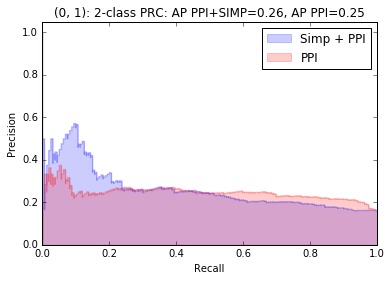
\includegraphics[width=\linewidth]{logisticRegressionGraphs/logr1.png}
\endminipage\hfill
\minipage{0.32\textwidth}
  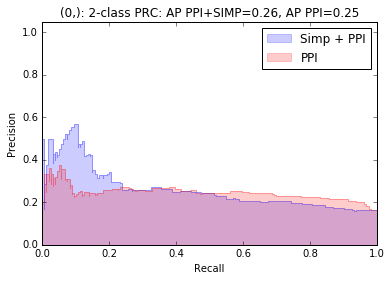
\includegraphics[width=\linewidth]{logisticRegressionGraphs/logr3.png}
\endminipage\hfill
\minipage{0.32\textwidth}%
  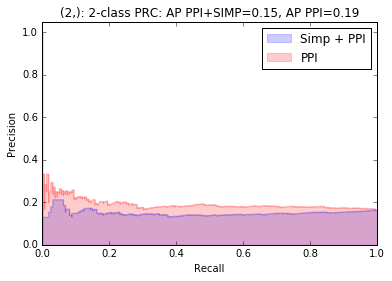
\includegraphics[width=\linewidth]{logisticRegressionGraphs/logr6.png}
\endminipage
\caption{Precision and Recall curves of different combinations of centralities for Logistic Regression}
\end{figure}
What above figures show, is the difference Precision and Recall curves for different combination of input and how the resulted logistic regression model performed in both ppi and simplicial complexes network. As we can notice, our maximum average precision over all the combination of input is 25\% in simplicial complexes and 22\% in PPI networks. Something else we can observe is that our precision drops really suddenly once we increase the recall. Which means, only very few instances are right if we want to be precise. Precision drops to a constant value and stays around it as the recall increases. It is clear that prediction capacity of this model is quite bad. Some combinations seems to perform better under simplicial complexes and some combinations performs worse.

\begin{figure}[!htb]
\minipage{0.32\textwidth}
  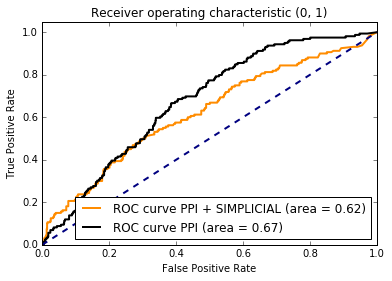
\includegraphics[width=\linewidth]{logisticRegressionGraphs/logr1S.png}
\endminipage\hfill
\minipage{0.32\textwidth}
  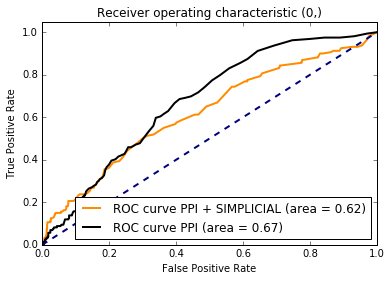
\includegraphics[width=\linewidth]{logisticRegressionGraphs/logr2S.png}
\endminipage\hfill
\minipage{0.32\textwidth}%
  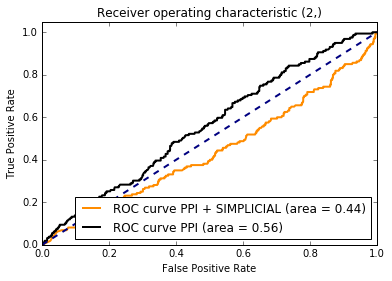
\includegraphics[width=\linewidth]{logisticRegressionGraphs/logr3S.png}
\endminipage
\caption{Receiver Operating Characteristic curves of Logistic Regression}
\end{figure}
Above shown Receiver Operating Characteristic (ROC) are plotted based on the combination of models we generated from different combinations of input. The dotted line represents the True and False positive output we get from a random classifier when we move the threshold of the prediction from high to low. The Orange curve, ROC curve, represents the True and False positive rate we would get from the models as we move our threshold. Even though three out of 7 models perform bit better than a random classifier, these model’s prediction power is quite low and have a high False positive rate. As we can see, some of the combinations have better True and False positive rate considering the area under the curve which shows how good a model performs. (First and third models have the area value of 0.66 which is more than the other combinations)

\subsection{Random Forest Classification}
\begin{figure}[!htb]
\minipage{0.32\textwidth}
  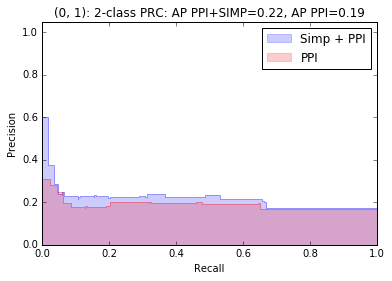
\includegraphics[width=\linewidth]{logisticRegressionGraphs/for1.png}
\endminipage\hfill
\minipage{0.32\textwidth}
  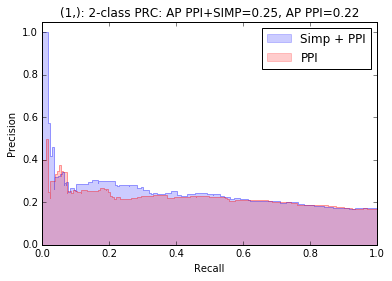
\includegraphics[width=\linewidth]{logisticRegressionGraphs/for2.png}
\endminipage\hfill
\minipage{0.32\textwidth}%
  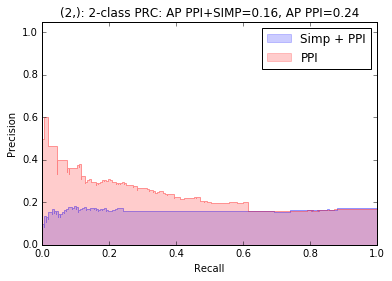
\includegraphics[width=\linewidth]{logisticRegressionGraphs/for3.png}
\endminipage
\caption{Precision and Recall curves of different combinations of centralities for Random Forest}
\end{figure}

Above figures depict different Precision and Recall curves for different combination of centrality inputs and how Random Forest Classification model performed in both ppi and simplicial complexes networks. According to the figures, maximum average precision over all the combinations of centralities as inputs is less than 20\% in ppi networks and simplicial complexes around 20\%. Also it is important to note that, some models seems to have a slower drop in precision in both Simplicial Complexes and PPI networks. We can see that simplicial complex models only perform better under certain combination of topological measures but the maximum average precision suggest that this enhancement in performance is not significant. For all the models, the precision barely increases as the recall increases and it’s almost constant after a certain recall in PPI networks.

\newpage
\begin{figure}[!htb]
\minipage{0.32\textwidth}
  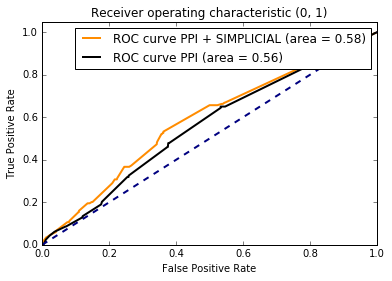
\includegraphics[width=\linewidth]{logisticRegressionGraphs/forS1.png}
\endminipage\hfill
\minipage{0.32\textwidth}
  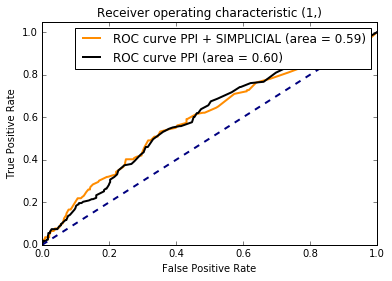
\includegraphics[width=\linewidth]{logisticRegressionGraphs/forS2.png}
\endminipage\hfill
\minipage{0.32\textwidth}%
  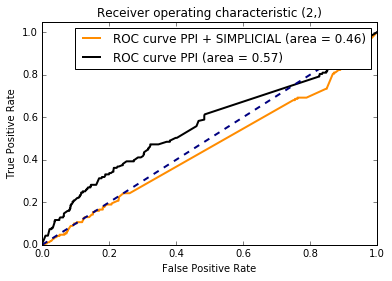
\includegraphics[width=\linewidth]{logisticRegressionGraphs/forS3.png}
\endminipage
\caption{Receiver Operating Characteristic curves of Random Forest}
\end{figure}
ROC curves for Random Forest Classification shows the similar performance, if not worse compared to the one we got for Logistic regression. On average, random forest classification gives us worse performance and worse average area under the curve. Also we can note that simplicial complexes do not perform better in some combinations of inputs as measures.

\subsection{Agglomerative Clustering}
\begin{figure}[!htb]
  \centering
  \minipage{0.7\textwidth}%
  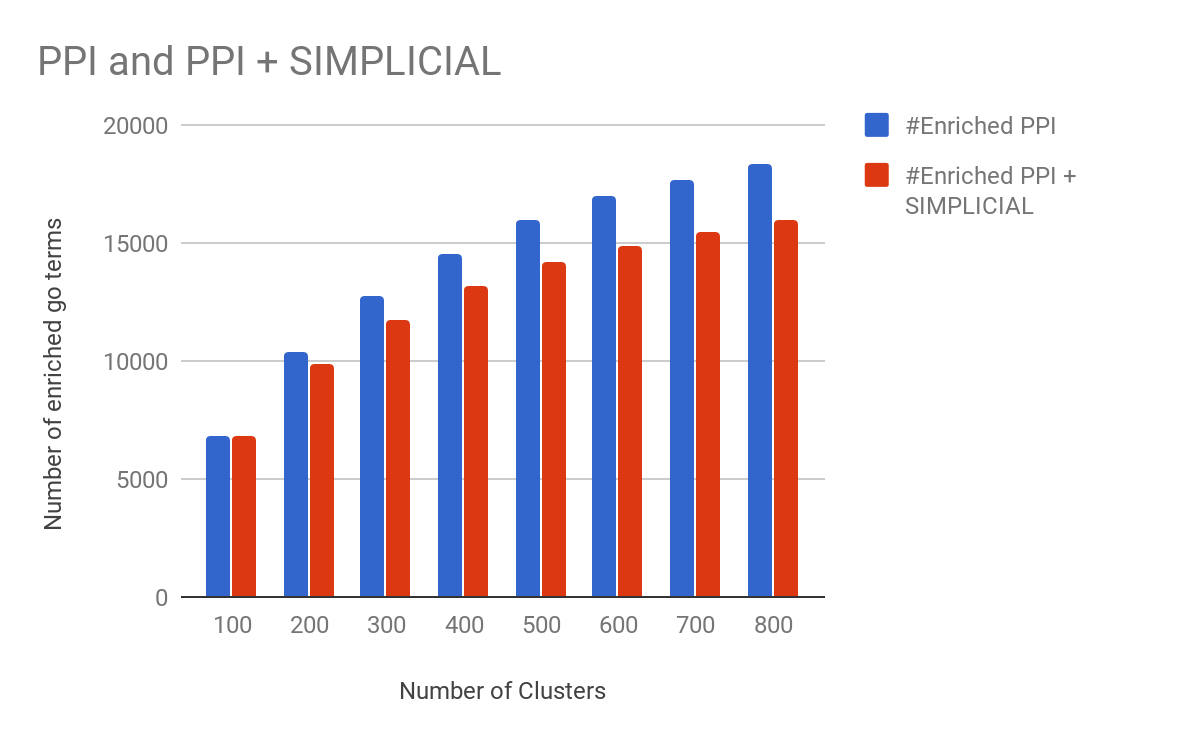
\includegraphics[width=\linewidth]{logisticRegressionGraphs/cluster.png}
\endminipage
\caption{Enrichment graph of PPI and Simplicial}
\end{figure}
We applied agglomerative clustering on the genes centrality data that we have collected on both ppi and simplicial complexes. We analysed each cluster to see if any of the GO terms are enriched in them. We calculated the p value for each GO term in each cluster for both ppi and simplicial complexes.\url{(https://www.nature.com/articles/srep35098\#supplementary-information)} We repeated the experiment by changing the number of clusters from 100 - 800 incrementing by 100 every time. The above figure depicts the number of clusters we have in the experiment and the number of enriched GO terms in that experiment. As we can see clustering based on all three centralities (betweenness, closeness and degree distribution) in simplicial complexes, did not give us more enriched GO terms. The figure also shows that as we increase the number of clusters, the number of enriched GO terms increases in both PPI and simplicial complexes. For future, this clustering may be used for predicting GO terms in the clusters. Also we can use combinations of centralities for our clustering model in future to see if we get better enrichments in both simplicial complexes and ppi networks. 

\section{Discussion \& Limitations} 
After placing the complexes data on top of the PPI network, in order to build the simplicial complex, we had 66,482 triangles in the network. For us to compute closeness centrality and betweenness centrality, we needed to calculate the shortest paths between each pair of triangles. As Floyd Warshall’s shortest path algorithm is \(O(N^3)\), and the number of edges in the simplicial complexes is well over 150 million, which was computationally exhaustive to calculate. A naive implementation could take easily 11 days for betweenness centrality to complete. Additionally, as all the algorithms we implemented were in Python, which is a higher level language with a lot more abstractions, it is in fact much slower than other lower level languages like C or C++. Furthermore, it is worth mentioning that because of the computation time, we were not able to apply our methods to higher dimensions, further than triangles, in simplicial complexes.
\par
To address this issue, instead of using our own implementation of centralities and shortest path algorithms for simplicial complexes, we used NetworkX library. In order for us to use this library, we had to model our triangular simplicial network as a binary network, which means that each triangle in the network would be considered a node and the edge list would be built accordingly. This made the calculation significantly faster because NetworkX implementations use APIs to compute general algorithms which are heavily optimised.
\par
Additionally, another constraint was that we had no access to any powerful computer clusters. Therefore, we were unable to continuously run our experiments as they became extremely time consuming to compute. Also, if we had access to clusters, since this project is heavily data-driven, parallelisation would have been effective in speeding up the computations required.  

\section{Conclusion and Future Work}
Our results from the regression model suggest that using multiple combinations of topological measures does not yield a performance gain in the resulting model, lead us to believe that the model performs poorly with the given data. We found out that logistic regression works better than linear regression on this data through. However, the issue with performance persists as seen in our precision and recall curves where the accuracy of the predictions is still quite low. Through the comparison of both PPI and simplicial complex on top of PPI, we were able to observe that the simplicial complex performed better. However, the conclusion is that the result of adding simplicial complex onto PPI doesn’t provide us with the performance advancement that we initially expected, and on contrary, it significantly worsens with higher false positives on some inputs. Another observation that we could make of this is that random forest classification performs worse than logistic regression, and the result of adding simplicial complexes were inconclusive. As a general trend, we noticed that models whose input involves betweenness seem to perform better with simplicial complexes rather than PPI network alone. Finally, the results from agglomerative clustering show that the addition of simplicial complexes gives us less enrichment upon clustering in comparison to PPI network alone, as illustrated in Figure WHATEVER; further disproving our hypothesis.
 
 
In future, we can improve our methodology by re-implementing the algorithms in a low-level language such as Java, C or C++ to reduce computation costs and runtime. This would be especially useful if we are considering nodes in higher dimensions as it would be more expensive computationally. Currently, we’ve only considered experimental GO IDs and this model can be used to check how well our predictions are performing on a real data set using the predicted GO-IDs in the Geneontology database. While clustering the data, one possible improvement can be clustering based different combinations of input. Taking away each input parameter and analysing how they perform based on other clustering and comparing Simplicial Complex versus PPI network. We can also validate the predicted enriched GO terms against different websites used for literature curation. It is also noted from the similar studies that, linkage methods for clustering has a significant impact on the resulting model. So experimenting with different linkage methods may result in a better output. Another feasible extension is to repeat the analysis on another complete dataset, eg. on human gene data.



\newpage
\begin{thebibliography}{8}
\bibitem{latexcompanion} 
Estrada, E. and Ross, G. (2018)
Centralities in simplicial complexes. Applications to protein interaction networks. Journal of Theoretical Biology, 438, pp.46-60

\bibitem{latexcompanion} 
Hahn, M. and Kern, A. (2004)
Comparative Genomics of Centrality and Essentiality in Three Eukaryotic Protein Interaction Networks. Molecular Biology and Evolution, 22(4), pp.803-806.

\bibitem{latexcompanion}
del Rio, G., Koschützki, D. and Coello, G. (2009). 
How to identify essential genes from molecular networks?. BMC Systems Biology, 3(1), p.102.

\bibitem{latexcompanion}
Chapter 4 of “Analysis of Biological Networks,“ edited by Bjorn J. Junker and Falk Schreiber, John Wiley \& Sons, 2008 

\bibitem{latexcompanion}
Wrzeszczynski, K., Ofran, Y., Rost, B., Nair, R. and Liu, J. (2003). Automatic prediction of protein function. Cellular and Molecular Life Sciences (CMLS), 60(12), pp.2637-2650.
 
\bibitem{techPapers} 
Cs.umn.edu. (2018). Browse Technical Reports, Computer Science \& Engineering. [online] Available at: \url{https://www.cs.umn.edu/research/technical_reports/view/06-028l} 

\bibitem{techWebsite}
Semanticscholar.org. (2018). A (not so) Quick Introduction to Protein Function Prediction - Semantic Scholar. [online] Available at: \url{https://www.semanticscholar.org/paper/A-(not-so)-Quick-Introduction-to-Protein-Function-Radivojac/d678f9a5e6e430b165b6a98f5fac2cfe66c3dc7c}

\bibitem{techwebsite}
Young, K. (2018). Yeast Two-hybrid: So Many Interactions, (in) So Little Time….
\url{https://academic.oup.com/biolreprod/article/58/2/302/2761050}

\bibitem{latexcompanion}
Gligorijević, V., Barot, M. and Bonneau, R. (2017). deepNF: Deep network fusion for protein function prediction. biorxiv preprint doi:10.1101/223339

\bibitem{latexcompanion}
Yu, D., Kim, M., Xiao, G. and Hwang, T. (2013). Review of Biological Network Data and Its Applications. Genomics \& Informatics, 11(4), p.200.

\bibitem{latexcompanion}
Andrade, M., Casari, G., de Daruvar, A., Sander, C., Schneider, R., Tamames, J., Valencia, A. and Ouzounis, C. (1997). Sequence analysis of the Methanococcus jannaschii genome and the prediction of protein function. Bioinformatics, 13(4), pp.481-483

\bibitem{latexcompanion}
Reeck, G. R.; de Haen, C.; Teller, D. C.; Doolittle, R. F.; Fitch, W. M.; Dickerson, R. E.; et al. (1987). ""Homology" in proteins and nucleic acids: a terminology muddle and a way out of it". Nature. 50 (5): 667.

\bibitem{latexcompanion}
EMBL-EBI Train online. (2018). Protein Classification. [online] Available at: \url{https://www.ebi.ac.uk/training/online/course/introduction-protein-classification-ebi/protein-classification}.

\bibitem{latexcompanion}
Zhao, H. (2018). Protein function prediction by integrating sequence, structure and binding affinity information. [online] Scholarworks.iupui.edu. Available at: \url{https://scholarworks.iupui.edu/handle/1805/3913}

\bibitem{latexcompanion}
Davis, D., Yaveroğlu, Ö., Malod-Dognin, N., Stojmirovic, A. and Pržulj, N. (2015). Topology-function conservation in protein–protein interaction networks. Bioinformatics, 31(10), pp.1632-1639.

\bibitem{latexcompanion}
Milenković T. Pržulj N. (2008) Uncovering biological network function via graphlet degree signatures. Cancer Inform. ,2008, 257–273.

\bibitem{latexcompanion}
Schwikowski, B., Uetz, P. and Fields, S. (2000). A network of protein–protein interactions in yeast. Nature Biotechnology, 18(12), pp.1257-1261.

\bibitem{latexcompanion}
Przulj N, Wigle DA, Jurisica I (2004) Functional topology in a network of protein interactions. Bioinformatics 20: 340–348

\bibitem{latexcompanion}
Chua, H., Sung, W. and Wong, L. (2006). Exploiting indirect neighbours and topological weight to predict protein function from protein-protein interactions. Bioinformatics, 22(13), pp.1623-1630.

\bibitem{latexcompanion}
Hishigaki, H., Nakai, K., Ono, T., Tanigami, A. and Takagi, T. (2001). Assessment of prediction accuracy of protein function from protein-protein interaction data. Yeast, 18(6), pp.523-531.

\bibitem{latexcompanion}
Sharan, R., Ulitsky, I. and Shamir, R. (2007). Network-based prediction of protein function. Molecular Systems Biology, 3.

\bibitem{latexcompanion}
Courtney, O. T., \& Bianconi, G. (2016). Generalized network structures: The configuration model and the canonical ensemble of simplicial complexes. Physical Review E, 93(6), 062311. 

\bibitem{latexcompanion}
Lab, M. (2018). BioGRID | Database of Protein, Chemical, and Genetic Interactions. [online] Thebiogrid.org. Available at: \url{https://thebiogrid.org/}

\bibitem{latexcompanion}
Gene Ontology Consortium (2018). The Gene Ontology (GO) database and informatics resource.

\bibitem{latexcompanion}
Wodaklab.org. (2018). About - CYC2008 - Wodak Lab. [online] Available at: \url{http://wodaklab.org/cyc2008/}

\bibitem{latexcompanion}
P. Tedder, J. Bradford, C. Needham, G. McConkey, A. Bulpitt and D. Westhead, "Gene function prediction using semantic similarity clustering and enrichment analysis in the malaria parasite Plasmodium falciparum", Bioinformatics, vol. 26, no. 19, pp. 2431-2437, 2010.

\bibitem{latexcompanion}
T. Hawkins, M. Chitale and D. Kihara, "Functional enrichment analyses and construction of functional similarity networks with high confidence function prediction by PFP", BMC Bioinformatics, vol. 11, no. 1, p. 265, 2010.

\bibitem{latexcompanion}
X. Zhou and Z. Su, "EasyGO: Gene Ontology-based annotation and functional enrichment analysis tool for agronomical species", BMC Genomics, vol. 8, no. 1, p. 246, 2007.

\bibitem{latexcompanion}
scikit-learn: machine learning in Python — scikit-learn 0.19.1 documentation, Scikit-learn.org, 2018. [Online]. Available: \url{http://scikit-learn.org/stable}

\bibitem{latexcompanion}
Www2.cs.duke.edu, 2018. [Online]. Available: \url{https://www2.cs.duke.edu/courses/fall06/cps296.1/Lectures/sec-III-1.pdf}

\bibitem{latexcompanion}
Centrality — NetworkX 1.10 documentation, Networkx.github.io, 2018. [Online]. Available: \url{https://networkx.github.io/documentation/networkx-1.10/reference/algorithms.centrality.html?highlight=centralities}

\bibitem{latexcompanion}
P. Tedder, J. Bradford, C. Needham, G. McConkey, A. Bulpitt and D. Westhead, "Gene function prediction using semantic similarity clustering and enrichment analysis in the malaria parasite Plasmodium falciparum", 2018. .

\bibitem{latexcompanion}
Petri Toronen, Ncbi.nlm.nih.gov, 2018. [Online]. Available: \url{https://www.ncbi.nlm.nih.gov/pmc/articles/PMC407846/pdf/1471-2105-5-32.pdf}

\bibitem{latexcompanion}
Pdfs.semanticscholar.org, 2018. [Online]. Available: \url{https://pdfs.semanticscholar.org/47c0/a7204e1ec5b48cde77ae12a99ac5d00be1be.pdf}

\bibitem{latexcompanion}
Ties in Proximity and Clustering Compounds

\bibitem{latexcompanion}
Freudenberg, J., Joshi, V., Hu, Z. and Medvedovic, M. (2009). CLEAN: CLustering Enrichment ANalysis. BMC Bioinformatics, 10(1), p.234.

\bibitem{latexcompanion}
Newman, M.E.J. 2010. Networks: An Introduction. Oxford, UK: Oxford University Press

\bibitem{latexcompanion}
Linton C. Freeman: Centrality in networks: I. Conceptual clarification. Social Networks 1:215-239, 1979

\bibitem{latexcompanion}
Ulrik Brandes: On Variants of Shortest-Path Betweenness Centrality and their Generic Computation. Social Networks 30(2):136-145, 2008

\bibitem{latexcompanion}
Pdfs.semanticscholar.org, 2018. [Online]. Available: \url{https://pdfs.semanticscholar.org/47c0/a7204e1ec5b48cde77ae12a99ac5d00be1be.pdf}
\end{thebibliography}




\end{document}
